\documentclass[12pt]{article}

\usepackage{breqn}
\usepackage[margin=1in]{geometry} 
\usepackage{amsmath,amsthm,amssymb,enumitem}
\usepackage[german,spanish,english]{babel}
\usepackage{tensor}
\usepackage{graphicx}
\usepackage{esint}
\usepackage[T1]{fontenc}
\usepackage{mathtools}
\usepackage{siunitx}
\usepackage[table,xcdraw]{xcolor}
\newenvironment{ex}[2][Exercise]{\begin{trivlist}
\item[\hskip \labelsep {\bfseries #1}\hskip \labelsep {\bfseries #2.}]}{\end{trivlist}}

\newenvironment{sol}[1][Solution]{\begin{trivlist}
\item[\hskip \labelsep {\bfseries #1:}]}{\end{trivlist}}

\newcommand{\meq}{\overset{!}{=}}
\DeclarePairedDelimiter\bra{\langle}{\rvert}
\DeclarePairedDelimiter\ket{\lvert}{\rangle}
\DeclarePairedDelimiterX\brk[2]{\langle}{\rangle}{#1\,\delimsize\vert\,\mathopen{}#2}
\DeclareSIUnit\angstrom{\text {Å}}

%DECLARATION OF DELIMITERS%

\DeclarePairedDelimiter\vb{\lvert}{\rvert}
\DeclarePairedDelimiter\rb{(}{)}
\DeclarePairedDelimiter\sqrb{[}{]}
\DeclarePairedDelimiter\cb{\{}{\}}
\DeclarePairedDelimiter\ab{\langle}{\rangle}
\DeclarePairedDelimiter\db{\|}{\|}


\begin{document}
\noindent Richard Abele \hfill \today \\[30pt]
\centerline{ \Large{ \textbf{ Numerical Methods - pset 4 }}}

\section{Problem 1}
\label{sec:prob1}

	

\subsection{Part A}
\label{subsec:prob1a}

\texttt{Part A} of \texttt{problem 1} requires the calculation of the Pade approximations \(P[3,4]\) and \(P[2,5]\) for the function \(f\rb*{x} = e^{x} \). To aid these calculations, Mathematica was used in calculating the Taylor expansion and derivatives. 

A Pade expansion \(R_{N}\rb*{x}\) takes the following form:
\begin{align*}
	f \rb*{x} & =  R_{N} \rb*{x} \equiv \frac{P_{n}\rb*{x}}{Q_{m}\rb*{x}} = 
	\frac{a_{0} + a_{1} x + a_{2}x^{2} + ... + a_{n}x^{n}}{
		1 + b_{1}x + b_{2}x^{2} + ... + b_{m}x^{m}
	}
\end{align*}
with \(N = n + m\).

Calculating a Pade approximation \(R_{3,4}\rb*{x}\) of \(f\rb*{x}\) requires first calculating the Maclaurin series of degree \(N = 3 + 4 = 2 + 5 = 7\) for \(f\rb*{x}\) (Taylor series about \(x=0\)). 
\begin{align*}
	f\rb*{x} & =  e^{x} &\\
	T_{7}\rb*{f\rb*{x}} & = 1 + x + \frac{x^{2}}{2} + \frac{x^{3}}{6} +
			    \frac{x^{4}}{24} + \frac{x^{5}}{120} + \frac{x^{6}}{720} + \frac{x^{7}}{5040}&\\
\end{align*}

We then create the difference
\begin{align*}
	T_{7}\rb*{x} - R_{3,m}\rb*{x} & =  0 &\\
	\Rightarrow \rb*{ T_{7}\rb*{x} }- 
	\frac{a_{0} + a_{1} x + a_{2}x^{2} + a_{3} x^{3}}{
		1 + b_{1}x + b_{2}x^{2} + ... + b_{m}x^{m}
	} & =  0 &\\
\end{align*}
Multipying out the denominator thus leads to 
\begin{align*}
	\frac{1}{1 + ... + b_{m}x^{m}} \sqrb*{T_{7}\rb*{x} \rb*{1 + b_{1}x + .. + b_{m}x^{m}} -
	\rb*{a_{0} + a_{1}x + a_{2}x^{2} + a_{3}x^{3}}} \\ = 0. &\\
\end{align*}
from which it follows
\begin{align*}
	T_{7}\rb*{x}\rb*{ 1 + b_{1}x + .. + b_{m}x^{m}} 
	= a_{0} + a_{1}x + a_{2}x^{2} + a_{3}x^{3}.
\end{align*}

Setting \(m = 4\) for the Pade approximation \(P[3,4]\) results in 
\begin{align*}
	T_{7}\rb*{x} \rb*{ 1 + b_{1}x + b_{2}x^{2} + b_{3}x^{3} + b_{4}x^{4}} 
	= a_{0} + a_{1}x + a_{2}x^{2} + a_{3}x^{3}.
\end{align*}

Multiplying out these polynomials and combining like terms leads the following system of eight equations:
\begin{align*}
	0 & =  1 - a_{0} &\\
	0 & = 1 + b_{1} - a_{1} &\\
	0 & =  \frac{1}{2} + b_{1} + b_{2} - a_{2} &\\
	0 & =  \frac{1}{6} + \frac{b_{1}}{2} + b_{2} + b_{3} - a_{3} &\\
	0 & =  \frac{1}{24} + \frac{b_{1}}{6} + \frac{b_{2}}{2} + b_{3} + b_{4} &\\
	0 & =  \frac{1}{120} + \frac{b_{1}}{4} + \frac{b_{2}}{6} + \frac{b_{3}}{2} + b_{4} &\\
	0 & =  \frac{1}{720} + \frac{b_{1}}{120} + \frac{b_{2}}{24} + \frac{b_{3}}{6} + \frac{b_{4}}{2} &\\
	0 & =  \frac{1}{5040} + \frac{b_{1}}{720} + \frac{b_{2}}{120} + \frac{b_{3}}{24} + \frac{b_{4}}{6} &\\
\end{align*}

Solving this system of equations using Mathematica yields the expected values for \(a\) and \(b\):
\begin{align*}
	a_{0} & =  1 &\\
	a_{1} & =  \frac{3}{7} &\\
	a_{2} & =  \frac{1}{14} &\\
	a_{3} & =  \frac{1}{210} &\\
	b_{1} & =  - \frac{4}{7} &\\
	b_{2} & =  \frac{1}{7} &\\
	b_{3} & =  - \frac{2}{105} &\\
	b_{4} & =  \frac{1}{840} &\\
\end{align*}

These values match the given Pade approximation, proving the relation as desired. 

The process for calculating \(P[2,5]\) is analogous:


\begin{align*}
	T_{7}\rb*{x}\rb*{ 1 + b_{1}x + .. + b_{m}x^{m}} 
	= a_{0} + a_{1}x + a_{2}x^{2}. &\\
	\Rightarrow 
	T_{7}\rb*{x}\rb*{ 1 + b_{1}x + b_{2} x^{2} + b_{3} x^{3} + b_{4} x^{4} + b_{5} x^{5}}  
	= a_{0} + a_{1}x + a_{2}x^{2}.
\end{align*}

The resulting system of equations is:

\begin{align*}
	0 & = 1 - a_{0} &\\
	0 & = 1 + b_{1} - a_{1} &\\
	0 & =  \frac{1}{2} + b_{1} + b_{2}  - a_{2} &\\
	0 & =  \frac{1}{6} + \frac{b_{1}}{2} + b_{2} + b_{3} &\\
	0 & =  \frac{1}{24} + \frac{b_{1}}{6} + \frac{b_{2}}{2} + b_{3} + b_{4} &\\
	0 & =  \frac{1}{120} + \frac{b_{1}}{24} + \frac{b_{2}}{6} + \frac{b_{3}}{2} + b_{4} + b_{5} &\\
	0 & =  \frac{1}{720} + \frac{b_{1}}{120} + \frac{b_{2}}{24} + \frac{b_{3}}{6} + \frac{b_{4}}{2} + b_{5} &\\
	0 & =  \frac{1}{5040} + \frac{b_{1}}{720} + \frac{b_{2}}{120} + \frac{b_{3}}{24} + \frac{b_{4}}{6} + \frac{b_{5}}{2} &\\
\end{align*}

Solving this system of equations using Mathematica once again yields the desired values for \(a\) and \(b\):

\begin{align*}
	a_{0} & =  1 &\\
	a_{1} & =  \frac{2}{7} &\\
	a_{2} & =  \frac{1}{42} &\\
	b_{1} & =  - \frac{5}{7} &\\
	b_{2} & =  \frac{5}{21} &\\
	b_{3} & =  - \frac{1}{21} &\\
	b_{4} & =  \frac{1}{168} &\\
	b_{5} & =  - \frac{1}{2520} &\\
\end{align*}

All three methods yield at least six decimal places of accuracy at \(x = 0.5\). This changes quickly after about \(x = 3.5\) at which point the functions take on very different values. 

At \(x = 2\) all three functions agree to at least 2 decimal places. At \(x = 5\), only the taylor approximation has the correct order of magnitude compared to the true value of the function and \(P[2,5]\) is even negative. 

     \begin{figure}[ht]
    \centering
    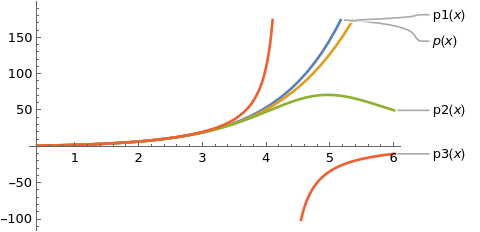
\includegraphics[width=0.75\textwidth]{graph_prob1.png}
    \caption{Graph of the original exponential function and the three different approximations}
    \label{fig:graph1}
\end{figure}



\section{Problem 2}
\label{sec:prob2}

For \texttt{problem 2} we are given four data points \(\rb*{x,y}\) and asked to find a third degree polynomial connecting these points. 

The provided table (seen below) also contains the calculated forward differences for the values. 


% Please add the following required packages to your document preamble:
% \usepackage[table,xcdraw]{xcolor}
% Beamer presentation requires \usepackage{colortbl} instead of \usepackage[table,xcdraw]{xcolor}
\begin{table}[h]
\begin{tabular}{llllll}
{\color[HTML]{323232} \(k\)} & {\color[HTML]{323232} \(x_{k}\)} & {\color[HTML]{323232} \(f\rb*{x_{k}}\)} & {\color[HTML]{323232} $\Delta f(x_k)$} & {\color[HTML]{323232} $\Delta ^2 f (x_k)$} & {\color[HTML]{323232} $\Delta ^3 f(x_k)$} \\
\hline
{\color[HTML]{323232} 0} & {\color[HTML]{323232} 4}   & {\color[HTML]{323232} 1}      & {\color[HTML]{323232} }              & {\color[HTML]{323232} }                  & {\color[HTML]{323232} }                 \\
{\color[HTML]{323232} }  & {\color[HTML]{323232} }    & {\color[HTML]{323232} }       & {\color[HTML]{323232} 2}             & {\color[HTML]{323232} }                  & {\color[HTML]{323232} }                 \\
{\color[HTML]{323232} 1} & {\color[HTML]{323232} 6}   & {\color[HTML]{323232} 3}      & {\color[HTML]{323232} }              & {\color[HTML]{323232} 3}                 & {\color[HTML]{323232} }                 \\
{\color[HTML]{323232} }  & {\color[HTML]{323232} }    & {\color[HTML]{323232} }       & {\color[HTML]{323232} 5}             & {\color[HTML]{323232} }                  & {\color[HTML]{323232} 4}                \\
{\color[HTML]{323232} 2} & {\color[HTML]{323232} 8}   & {\color[HTML]{323232} 8}      & {\color[HTML]{323232} }              & {\color[HTML]{323232} 7}                 & {\color[HTML]{323232} }                 \\
{\color[HTML]{323232} }  & {\color[HTML]{323232} }    & {\color[HTML]{323232} }       & {\color[HTML]{323232} 12}            & {\color[HTML]{323232} }                  & {\color[HTML]{323232} }                 \\
{\color[HTML]{323232} 3} & {\color[HTML]{323232} 10}  & {\color[HTML]{323232} 20}     & {\color[HTML]{323232} }              & {\color[HTML]{323232} }                  & {\color[HTML]{323232} }                
\end{tabular}
\end{table}

Given that these values are in order and equally spaced, we can use the following simplified formula to calcuate the Newton forward differences polynomial from the given values:

\begin{align*}
	P \rb*{x} & =  \sum_{i = 0}^{n} {\begin{pmatrix}
		s\\
		i
	\end{pmatrix}} \Delta ^{i} f_{0},
\end{align*}
with \(h\) being the spacing between the \(x\)-values and \(s = \frac{x - x_{0}}{h}\).

We can thus use the following expression to obtain the desired polynomial of degree three:
\begin{align*}
	P_{3} \rb*{x} & =  f_{0} + s \Delta f_{0} + \frac{s \rb*{s - 1}}{2 !} \Delta ^{2} f_{0} + \frac{s \rb*{s-1} \rb*{s - 2}}{3!} \Delta ^{3} f_{0} &\\
\end{align*}

We insert \(h = 2\) and the above expression for \(s\), as well as the forward finite differences to obtain the following (calculations done using Mathematica):

\begin{align*}
	P_{3} \rb*{x} & = \frac{x^{3}}{12} - \frac{9 x^{2}}{8} + \frac{71 x}{12} - 10, &\\
\end{align*}
which matches the given expression. 



\end{document}
